%!TEX root = paper.tex
\section{Countermeasures and Responses}
\label{sec:hiding}
This work is a single snapshot in an evolving landscape of attacks on payment systems. While Bluetana has
proven effective at finding Bluetooth skimmers, it by no means represents the last move in the cat-and-mouse game. In
the remainder of this section, we discuss what the next few steps in this arms race might look like. That is, given
that inspectors and volunteers are using Bluetana, what can be the skimmer installers' next move, its cost, and what our
response might be. It is possible for a determined and resourceful criminal to implement the countermeasures that we will be describing (particularly non-discoverable mode).


\subsection{Switching to Bluetooth Low Energy}
\label{sec:hiding:ble}

We have observed that by switching to BLE, criminals have \emph{many} more places to hide.
%
Figure~\ref{fig:classic-v-ble} shows the cumulative distribution of the number of BLE and Bluetooth devices we saw at each
fuel station.
%
Under the filtering of Section~\ref{sec:bluetooth}, over 8,000 unique BLE devices were seen, making
the ratio of Classic to BLE approximately 1:4.

\begin{figure}
    \centering
    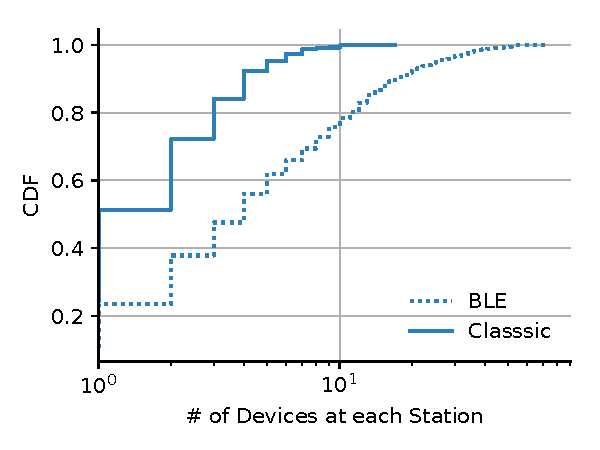
\includegraphics[width=0.6\linewidth]{skimmer/plots/cdf_num_devices_seen.pdf}
    \caption{BLE devices are more common than Classic.}
    \label{fig:classic-v-ble}
    \vspace{-1em}
\end{figure}

\paragraph{Cost to attacker} There is almost no cost to criminals in switching their Bluetooth modules to BLE.
%
In fact, newer EMV skimmers discovered in other countries are BLE enabled~\cite{krebshimmer}.
%
However, none of our contacts in law enforcement have encountered BLE-based gas station skimmers.
%
It is possible that there is simply no incentive to switch: the same reason criminals have not yet adapted to
masking their Bluetooth device class.

\paragraph{Response} BLE devices may be harder to differentiate due to the higher number of devices at each gas
station and a lack of distinguishing features.
%
With more sophisticated filtering techniques, it may still be possible to isolate BLE skimmers within
this larger set of devices.
%
One possibility is automated RSSI localization to the fuel dispenser location, a possible subject of future research.

\subsection{Non-Discoverable Skimmers}
\label{sec:hiding:desc}

The most natural way to evade discovery via Bluetooth would be to put the module in non-discoverable mode.
%
When a Bluetooth device is non-discoverable, it does not respond to normal Bluetooth scans.
%
Instead, it only responds to paging packets specifically addressed to its MAC address.

\paragraph{Cost to attacker} Non-discoverability would make exfiltration more difficult for criminals.
%
One possibility is creating a pre-paired data collection device.
%
However, we have been informed by law enforcement that the individual who installs the skimmer is often independent
from the individual responsible for data recovery (called a ``mule'').
%
The criminal would not be able to send a mule to recover card data without first delivering them the device.
%
Alternately the criminal could record the MAC address of the skimmer Bluetooth module.
%
This would require careful bookkeeping and the use of tools that support the creation of a non-discoverable connection.

\begin{comment}
    The downside of pre-pairing and making the device non-discoverable is that the device
    becomes visible \emph{only} to the host with which it was pre-paired. This means that the person sent to collect the
    skimmer data must have the same host device with which the skimmer has been paired before installation. Moreover, if
    this host device is lost or becomes nonfunctional, all access to the skimmer is lost. The installer would need to
    physically access the skimmer to initiate pairing again, which carries nearly the same risk as installing a new
    skimmer.
\end{comment}

\paragraph{Response} It is still possible to discover a non-discoverable device.
%
For a small set of target address ranges, e.g., \texttt{00:06:66} used by Roving Networks modules, we believe it
would be practical to attempt to guess all 16.8 million possible addresses.
%
Prior work has shown that it is possible to discover any non-discoverable device via brute force in 18.64 hours;
knowledge of OUI would ideally allow us to reduce this search time~\cite{cross2007detecting}.
%
Unfortunately, this requires specialized hardware, rather than an inexpensive Android phone.

\subsection{Impersonating Common Benign Devices}
Another natural response to Bluetana would be to change the MAC address and name of the device to that of a common
benign device, such as a mobile phone or a Bluetooth-enabled car entertainment system. This would make the skimmer
appear innocuous to Bluetana.

\paragraph{Cost to attacker} Reprogramming the MAC address on the CSR-based Bluetooth modules, which include the
Roving Networks and HC-05 and HC-06 modules, cannot be done using the AT commands used to change device name and
pairing. Instead, the skimmer installer would need to re-flash the CSR firmware using a special programming cable.
While, in principle, not difficult, it would require an additional degree of sophistication than programming a simple
micro-controller development board. The skimmer installer could also change the device name but not the MAC address,
say, to one of the known benign devices using the same module, something that us possible to do by issuing AT
commands from the micro-controller to the module. While this may cause Bluetana to detect these as a skimmer, signal strength can still be used to identify location of the module.

\paragraph{Response} Because Bluetana collects all Bluetooth data, we can identify skimmers retroactively when we
learn of a new MAC address and name used by known skimmers. Thus, if attacks switch to impersonating benign devices,
we can update the Bluetana highlighting mechanism to identify those devices as suspicious. This would result in
additional inspections, but would still provide significant gain over the state of the art.

\subsection{Using Non-Bluetooth Communications}
During discussions with law enforcement agencies tasked with identifying skimmers, we were told about skimmers that
use GSM modems or WiFi as an alternative to Bluetooth. In the case of WiFi, we believe that the Bluetana methodology
will still be effective. GSM poses a more serious challenge for detection.

\paragraph{Cost to attacker}
While using GSM would avoid detection using Bluetana, it creates an additional trail of evidence linking the
perpetrator to the skimmer. Law enforcement officers could obtain information about the SMS recipient through
subpoenas, so receiving the SMS messages on another phone on a US carrier, for example, would be easy to trace.The
perpetrator would need to use an SMS service that would not expose his/her identity.

\paragraph{Response} In addition to legal tools available to law enforcement to trace SMS messages, a GSM modem could
be detected using a Software-Defined Radio.% including a low-cost (\$10) RTL-SDR dongle.

\subsection{Attacker Bottlenecks}
The attacker (skimmer installer) has several practical ways to evade detection using Bluetana. Each of these, however
, has an additional cost to the attacker in terms of effort, risk exposure, or expertise. We do not yet have a strong
understanding to which of these costs attackers are most sensitive. Indeed, the very low price of stolen credit card
numbers, compared to their potential cash out value (Table~\ref{tab:cardval}) suggests that the bottleneck in the
carding value chain is \emph{not} getting card information but cashing out cards. Thus, while Bluetana may raise the
cost for attackers, we do not believe that it will raise it so much as to make fuel dispenser skimming unprofitable.
